% Options for packages loaded elsewhere
\PassOptionsToPackage{unicode}{hyperref}
\PassOptionsToPackage{hyphens}{url}
\PassOptionsToPackage{dvipsnames,svgnames,x11names}{xcolor}
%
\documentclass[
  number]{elsarticle}

\usepackage{amsmath,amssymb}
\usepackage{iftex}
\ifPDFTeX
  \usepackage[T1]{fontenc}
  \usepackage[utf8]{inputenc}
  \usepackage{textcomp} % provide euro and other symbols
\else % if luatex or xetex
  \usepackage{unicode-math}
  \defaultfontfeatures{Scale=MatchLowercase}
  \defaultfontfeatures[\rmfamily]{Ligatures=TeX,Scale=1}
\fi
\usepackage{lmodern}
\ifPDFTeX\else  
    % xetex/luatex font selection
\fi
% Use upquote if available, for straight quotes in verbatim environments
\IfFileExists{upquote.sty}{\usepackage{upquote}}{}
\IfFileExists{microtype.sty}{% use microtype if available
  \usepackage[]{microtype}
  \UseMicrotypeSet[protrusion]{basicmath} % disable protrusion for tt fonts
}{}
\makeatletter
\@ifundefined{KOMAClassName}{% if non-KOMA class
  \IfFileExists{parskip.sty}{%
    \usepackage{parskip}
  }{% else
    \setlength{\parindent}{0pt}
    \setlength{\parskip}{6pt plus 2pt minus 1pt}}
}{% if KOMA class
  \KOMAoptions{parskip=half}}
\makeatother
\usepackage{xcolor}
\setlength{\emergencystretch}{3em} % prevent overfull lines
\setcounter{secnumdepth}{5}
% Make \paragraph and \subparagraph free-standing
\makeatletter
\ifx\paragraph\undefined\else
  \let\oldparagraph\paragraph
  \renewcommand{\paragraph}{
    \@ifstar
      \xxxParagraphStar
      \xxxParagraphNoStar
  }
  \newcommand{\xxxParagraphStar}[1]{\oldparagraph*{#1}\mbox{}}
  \newcommand{\xxxParagraphNoStar}[1]{\oldparagraph{#1}\mbox{}}
\fi
\ifx\subparagraph\undefined\else
  \let\oldsubparagraph\subparagraph
  \renewcommand{\subparagraph}{
    \@ifstar
      \xxxSubParagraphStar
      \xxxSubParagraphNoStar
  }
  \newcommand{\xxxSubParagraphStar}[1]{\oldsubparagraph*{#1}\mbox{}}
  \newcommand{\xxxSubParagraphNoStar}[1]{\oldsubparagraph{#1}\mbox{}}
\fi
\makeatother


\providecommand{\tightlist}{%
  \setlength{\itemsep}{0pt}\setlength{\parskip}{0pt}}\usepackage{longtable,booktabs,array}
\usepackage{calc} % for calculating minipage widths
% Correct order of tables after \paragraph or \subparagraph
\usepackage{etoolbox}
\makeatletter
\patchcmd\longtable{\par}{\if@noskipsec\mbox{}\fi\par}{}{}
\makeatother
% Allow footnotes in longtable head/foot
\IfFileExists{footnotehyper.sty}{\usepackage{footnotehyper}}{\usepackage{footnote}}
\makesavenoteenv{longtable}
\usepackage{graphicx}
\makeatletter
\def\maxwidth{\ifdim\Gin@nat@width>\linewidth\linewidth\else\Gin@nat@width\fi}
\def\maxheight{\ifdim\Gin@nat@height>\textheight\textheight\else\Gin@nat@height\fi}
\makeatother
% Scale images if necessary, so that they will not overflow the page
% margins by default, and it is still possible to overwrite the defaults
% using explicit options in \includegraphics[width, height, ...]{}
\setkeys{Gin}{width=\maxwidth,height=\maxheight,keepaspectratio}
% Set default figure placement to htbp
\makeatletter
\def\fps@figure{htbp}
\makeatother

\makeatletter
\@ifpackageloaded{caption}{}{\usepackage{caption}}
\AtBeginDocument{%
\ifdefined\contentsname
  \renewcommand*\contentsname{Table of contents}
\else
  \newcommand\contentsname{Table of contents}
\fi
\ifdefined\listfigurename
  \renewcommand*\listfigurename{List of Figures}
\else
  \newcommand\listfigurename{List of Figures}
\fi
\ifdefined\listtablename
  \renewcommand*\listtablename{List of Tables}
\else
  \newcommand\listtablename{List of Tables}
\fi
\ifdefined\figurename
  \renewcommand*\figurename{Figure}
\else
  \newcommand\figurename{Figure}
\fi
\ifdefined\tablename
  \renewcommand*\tablename{Table}
\else
  \newcommand\tablename{Table}
\fi
}
\@ifpackageloaded{float}{}{\usepackage{float}}
\floatstyle{ruled}
\@ifundefined{c@chapter}{\newfloat{codelisting}{h}{lop}}{\newfloat{codelisting}{h}{lop}[chapter]}
\floatname{codelisting}{Listing}
\newcommand*\listoflistings{\listof{codelisting}{List of Listings}}
\makeatother
\makeatletter
\makeatother
\makeatletter
\@ifpackageloaded{caption}{}{\usepackage{caption}}
\@ifpackageloaded{subcaption}{}{\usepackage{subcaption}}
\makeatother
\ifLuaTeX
  \usepackage{selnolig}  % disable illegal ligatures
\fi
\usepackage[]{natbib}
\bibliographystyle{elsarticle-num}
\usepackage{bookmark}

\IfFileExists{xurl.sty}{\usepackage{xurl}}{} % add URL line breaks if available
\urlstyle{same} % disable monospaced font for URLs
\hypersetup{
  pdftitle={Seagrass mapping in two mudflats in the Auray River},
  pdfauthor={Simon Oiry; Bede Ffinian Rowe Davies},
  pdfkeywords={Remote Sensing, Sentinel-2, Seagrass},
  colorlinks=true,
  linkcolor={blue},
  filecolor={Maroon},
  citecolor={Blue},
  urlcolor={Blue},
  pdfcreator={LaTeX via pandoc}}

\setlength{\parindent}{6pt}
\begin{document}

\begin{frontmatter}
\title{Seagrass mapping in two mudflats in the Auray
River \\\large{About a rapid evolution of seagrasses} }
\author[1]{Simon Oiry%
\corref{cor1}%
}
 \ead{oirysimon@gmail.com} 
\author[1]{Bede Ffinian Rowe Davies%
\corref{cor1}%
}
 \ead{bedeffinian@gmail.com} 

\affiliation[1]{organization={Nantes Université, UR 2160, F-44000
Nantes, France, Institut des Substances et Organismes de la Mer,
ISOMer},addressline={2 chemin de la
houssinière},city={Nantes},postcode={44300},postcodesep={}}

\cortext[cor1]{Corresponding author}


        
\begin{abstract}
Maps of seagrass in two sites in the Auray River. These two sites were
studied by Maxime Daviray during his PhD. Seagrass appeared very quickly
during his PhD. This work aims to describe this rapid evolution of
seagrasses.
\end{abstract}





\begin{keyword}
    Remote Sensing \sep Sentinel-2 \sep 
    Seagrass
\end{keyword}
\end{frontmatter}
    
The data and scripts used for this work can be found
\href{https://github.com/SigOiry/Seagrass_maps_Maxime}{here}.

\section{Materials \& Methods}\label{materials-methods}

\subsection{Seagrass mapping using
Sentinel-2}\label{seagrass-mapping-using-sentinel-2}

To map the seagrass extent over time, the Sentinel-2 constellation has
been used. Level-2 images, which are already orthorectified and
atmospherically corrected, have been downloaded using the Copernicus
Platform \citep{Copernicus_Sentinel}. One low tide, cloud-free image per
year, nearest to the period of the annual maximum seagrass biomass at
this latitude has been used. A total of 8 images have been used
(Table~\ref{tbl-tide-data}).

\begin{longtable}[]{@{}
  >{\centering\arraybackslash}p{(\columnwidth - 4\tabcolsep) * \real{0.3194}}
  >{\centering\arraybackslash}p{(\columnwidth - 4\tabcolsep) * \real{0.2778}}
  >{\centering\arraybackslash}p{(\columnwidth - 4\tabcolsep) * \real{0.4028}}@{}}
\caption{Acquisition dates of Sentinel-2 images used to map seagrass in
the Auray River mudflats. Tide times were retrieved from the SHOM and
correspond to the tides at the Locmariaquer tide gauge, situated
approximately 2 km from the study
sites.}\label{tbl-tide-data}\tabularnewline
\toprule\noalign{}
\begin{minipage}[b]{\linewidth}\centering
Acquisition Date (UTC)
\end{minipage} & \begin{minipage}[b]{\linewidth}\centering
Low Tide Time (UTC)
\end{minipage} & \begin{minipage}[b]{\linewidth}\centering
Time Difference with Low tide
\end{minipage} \\
\midrule\noalign{}
\endfirsthead
\toprule\noalign{}
\begin{minipage}[b]{\linewidth}\centering
Acquisition Date (UTC)
\end{minipage} & \begin{minipage}[b]{\linewidth}\centering
Low Tide Time (UTC)
\end{minipage} & \begin{minipage}[b]{\linewidth}\centering
Time Difference with Low tide
\end{minipage} \\
\midrule\noalign{}
\endhead
\bottomrule\noalign{}
\endlastfoot
2016-11-03 11:12 & 12 : 08 & + 00 : 56 \\
2017-10-04 11:08 & 09 : 09 & - 01 : 59 \\
2018-09-29 11:08 & 12 : 43 & + 01 : 35 \\
2019-09-14 11:06 & 10 : 28 & + 00 : 38 \\
2020-08-04 11:06 & 10 : 45 & + 00 : 21 \\
2021-10-08 11:09 & 11 : 18 & - 00 : 09 \\
2022-08-29 11:06 & 11 : 27 & - 00 : 21 \\
2023-09-03 11:06 & 12 : 28 & - 01 : 22 \\
\end{longtable}

The \emph{Intertidal Classification of Europe: Categorising Reflectance
of Emerged Areas of Marine vegetation with Sentinel-2} model has been
applied to each Sentinel-2 image (ICE CREAMS, \citep{Davies2024}). It is
a neural network classifier designed to identify and discriminate
intertidal vegetation in Europe. Pixels of the Magnoliopsida class
(seagrasses) have been isolated, and the Normalized Difference
Vegetation Index (NDVI, \citep{rouse1974monitoring}), a commonly used
remote sensing biomass proxy for vegetation, has been employed. The
equation of \citep{zoffoli2020sentinel} have been used to transform NDVI
values into Seagrass Percent Cover (Equation~\ref{eq-std}). Only pixels
with SPC values above 20\%, corresponding to high biomass pixel have
been considered in order to avoid confusion with other class of
vegetation.

\begin{equation}\phantomsection\label{eq-std}{
SPC = 172.06 \times NDVI - 22.18
}\end{equation}

Maps and analysis have then been performed using the \emph{Terra}
package of R, in a \emph{Tidyverse} workflow
\citep{hijmans2023terra, wickham2017easily}.

\section{Results}\label{results}

\subsection{Evolution of the spatial distribution of seagrasses over
time}\label{evolution-of-the-spatial-distribution-of-seagrasses-over-time}

The time series of the seagrass percent cover between 2016 and 2023
shows an overall increase in meadow extent at both
sites(Figure~\ref{fig-Maps}). From 2019 onwards, the meadows became
denser at Fort Espagnol, particularly in the northern part of the
mudflat. At Kerouarc'h, the meadow was limited to small, sparse patches
between 2016 and 2019. However, from 2021 onward, the seagrass meadow
experienced a rapid expansion, covering almost the entire mudflat.

\phantomsection\label{cell-fig-Maps}
\begin{figure}[H]

\centering{

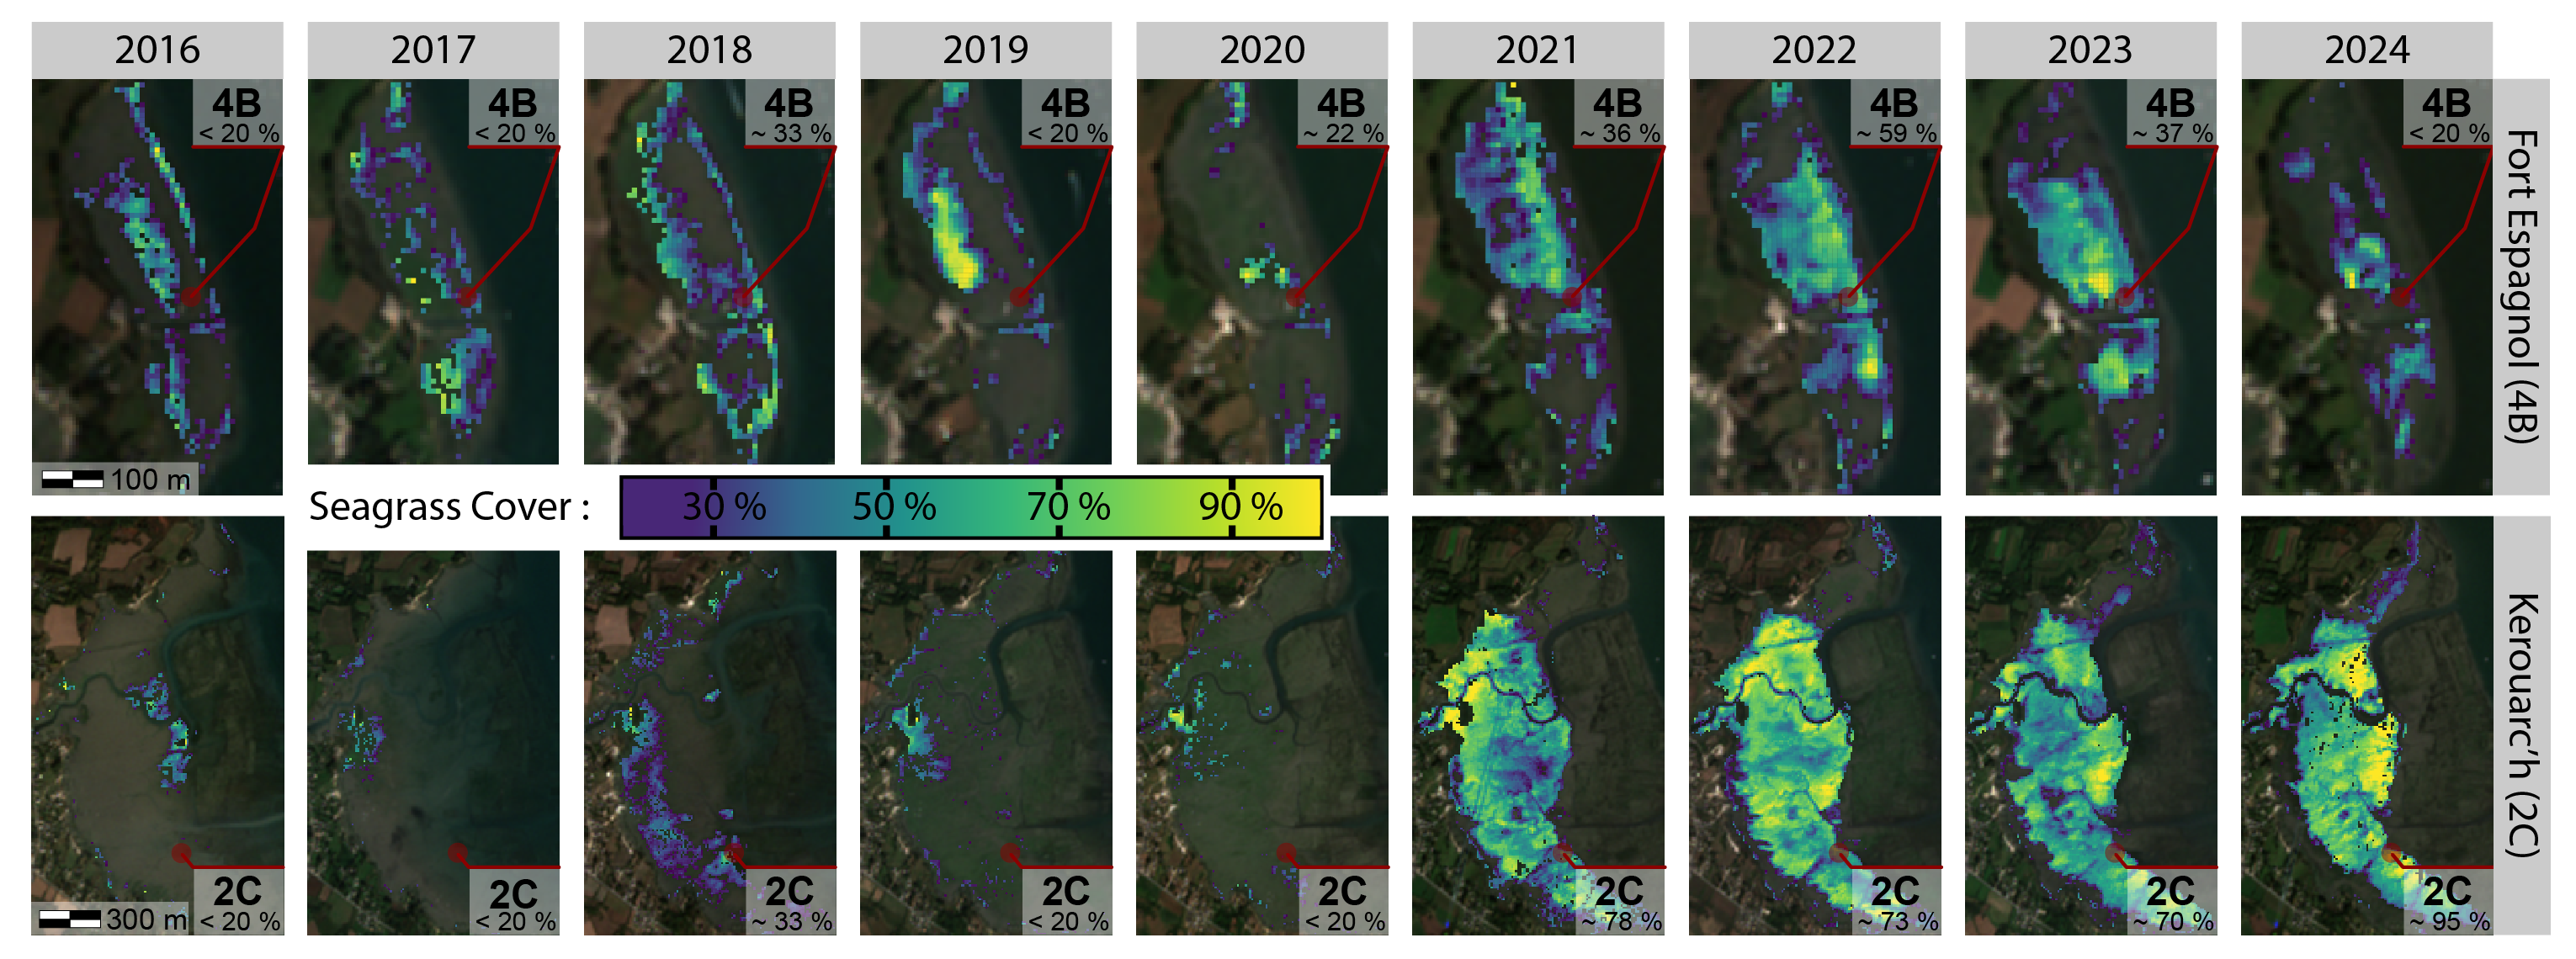
\includegraphics[width=1\textwidth,height=\textheight]{../Output/Figs/Figure1.png}

}

\caption{\label{fig-Maps}Time Serie of the Seagrass Percent cover
between 2016 and 2023 in Fort Espagnol and Kerouarc'h, two sites of the
Auray river.}

\end{figure}%

\subsection{Evolution of the extent and density of the meadow over
time}\label{evolution-of-the-extent-and-density-of-the-meadow-over-time}

The maximum total extent of seagrass was reached in 2021 at Fort
Espagnol and in 2022 at Kerouarc'h. Overall, during this period, the
extent of the meadow at Fort Espagnol increased by approximately 50\%
and by about 90\% at Kerouarc'h (Figure~\ref{fig-Extent} A). The density
of the meadow remained relatively constant between 2016 and 2020 at both
sites before increasing to 54\% of the median SPC in 2023 at Fort
Espagnol and 63\% in 2022 at Kerouarc'h (Figure~\ref{fig-Extent} B). The
year 2020 is an exception to these trends due to green algae covering
the meadow in August, which impeded the detection of the underlying
seagrass with remote sensing techniques.

\phantomsection\label{cell-fig-Extent}
\begin{figure}[H]

\centering{

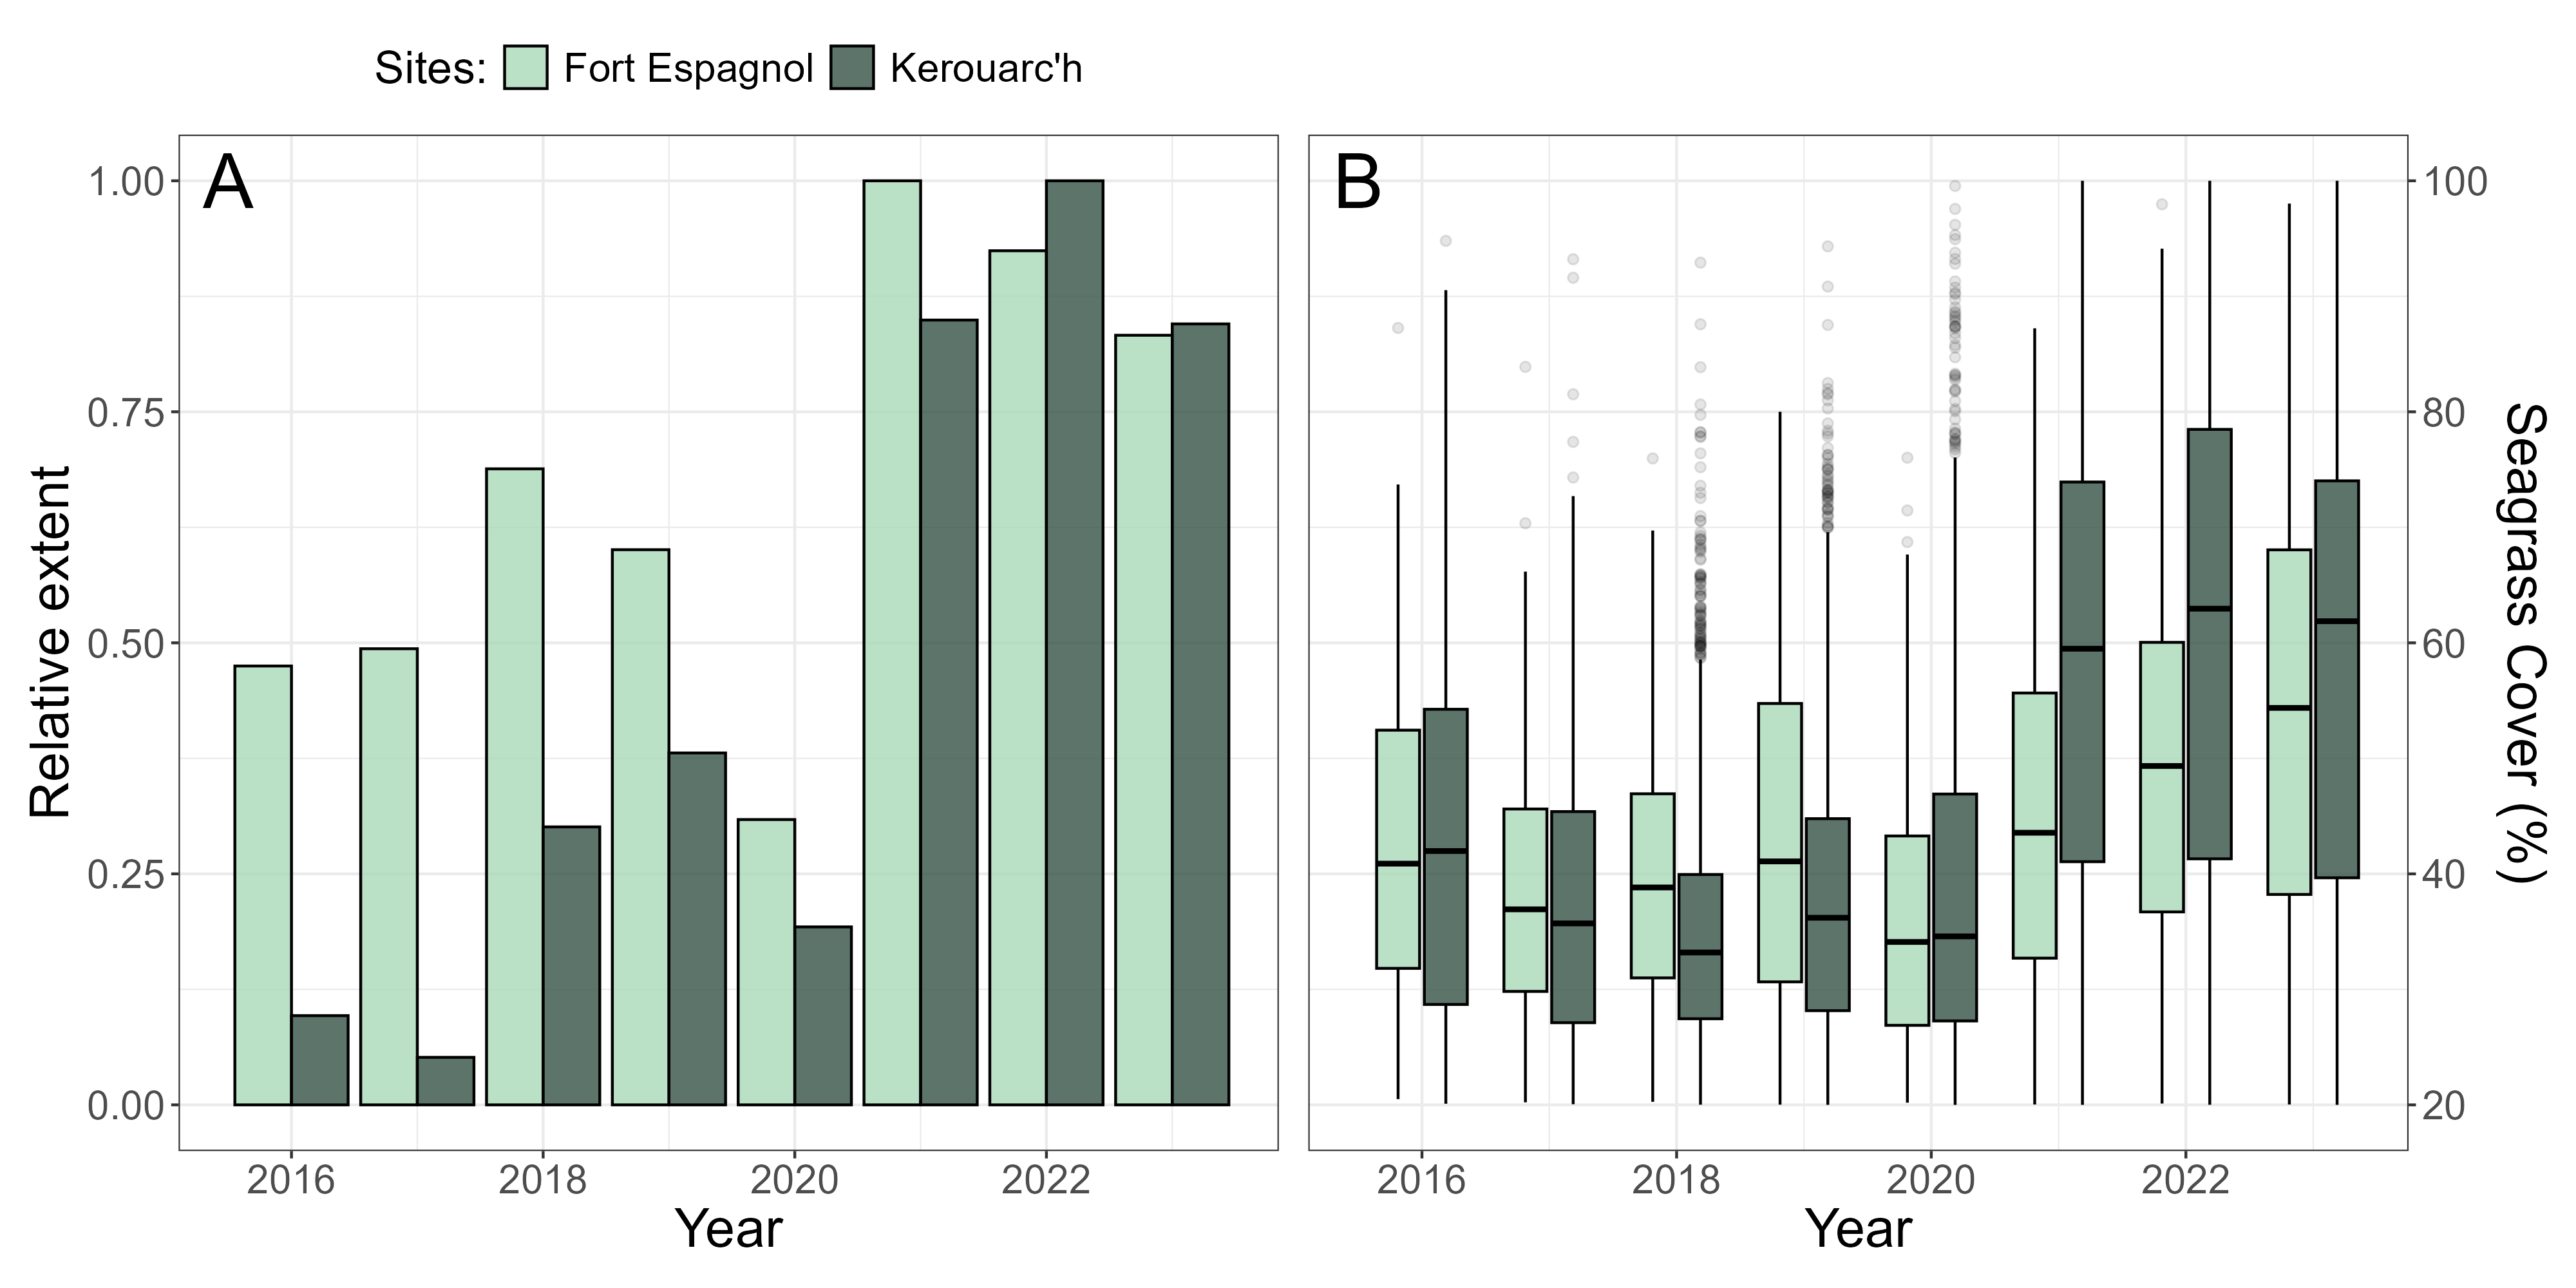
\includegraphics[width=1\textwidth,height=\textheight]{../Output/Figs/Figure2.png}

}

\caption{\label{fig-Extent}Descritpion of the evolution of seagrass over
time. A - Relative sesgrass extent of each site. 1 means maximum extent
of the time serie for the site. B - Boxplot of the density of seagrass
for each site at each date. The lower and upper hinges correspond to the
first and third quartiles (the 25th and 75th percentiles). Whiskers are
to 1.5 * IQR (Inter-Quartile Range) from the hinge.}

\end{figure}%


  \bibliography{library.bib}


\end{document}
